\documentclass[conference]{IEEEtran}
\usepackage[utf8]{inputenc}
\usepackage{graphicx}
\usepackage{amsmath}
\usepackage{cite}

\title{Reconocimiento de Placas Vehiculares Peruanas en Ruta: Dataset Propio y Modelo de Dos Etapas}

\author{
  \IEEEauthorblockN{Joel Ibaceta}
  \IEEEauthorblockA{
    \textit{Universidad Nacional de Ingeniería} \\
    joel.ibaceta.c@uni.pe
  }
  \and
  \IEEEauthorblockN{Marco Antonio Barrera Ninamango}
  \IEEEauthorblockA{
    \textit{Universidad Nacional de Ingeniería} \\
    marco.barrera.n@uni.pe
  }
  \and
  \IEEEauthorblockN{Jesus Gianpierre Campos Cardenas}
  \IEEEauthorblockA{
    \textit{Universidad Nacional de Ingeniería} \\
    j.campos.c@uni.pe
  }
}


\begin{document}

\maketitle

\begin{abstract}
Los sistemas de reconocimiento automático de placas vehiculares (ALPR) han alcanzado altos niveles de precisión en contextos controlados, pero presentan una significativa degradación de desempeño en entornos reales no estructurados, caracterizados por variabilidad en las condiciones de iluminación, movimiento de cámara y diversidad de configuraciones vehiculares. Esta problemática se agudiza en países como Perú, donde se observan particularidades adicionales como placas laterales pintadas, formatos extendidos y elementos visuales atípicos. En este trabajo se propone un enfoque jerárquico en dos etapas para la detección robusta de placas: primero se segmentan las regiones vehiculares utilizando un modelo YOLOv7 entrenado sobre una adaptación del conjunto de datos KITTI; posteriormente, se ejecuta una detección localizada de placas sobre dichas regiones, restringiendo el contexto visual y reduciendo la tasa de falsos positivos. Adicionalmente, se introduce un conjunto de datos curado manualmente a partir de grabaciones reales, anotado mediante un proceso asistido por OCR. Los resultados experimentales evidencian mejoras sustanciales en escenarios complejos, permitiendo identificar placas poco convencionales y múltiples instancias simultáneas en escenas densas de tráfico.
\end{abstract}

\hspace{0.5cm}

\section{Introducción}

El reconocimiento automático de placas vehiculares (ALPR) es ampliamente utilizado en control vehicular y seguridad pública. Sin embargo, su desempeño se ve limitado cuando se aplica en contextos distintos al de su entrenamiento original. En el caso peruano, modelos como ALPR-Unconstrained presentan errores al enfrentar placas con elementos particulares como la palabra “PERÚ”, o al confundirse con calcomanías y textos en el parabrisas. Además, muestran dificultades al operar desde una perspectiva frontal y móvil, típica de patrullaje o monitoreo embarcado, a diferencia de la vista elevada de muchos datasets disponibles.

La mayoría de estos modelos han sido entrenados con cámaras fijas y condiciones de iluminación controladas, lo que limita su capacidad de generalización a escenarios dinámicos. No obstante, el contexto local ofrece oportunidades únicas: en Perú, varios vehículos cuentan con placas pintadas en los laterales o parte trasera, que pueden servir como fuente redundante cuando la placa principal no es visible.

Este trabajo propone una solución adaptada a estas condiciones. Se presenta un nuevo dataset capturado desde la perspectiva del conductor, curado manualmente, junto con un modelo de detección entrenado sobre estas imágenes. El enfoque apunta a mejorar la robustez en escenarios reales de monitoreo en movimiento, donde los sistemas tradicionales fallan.


\section{Trabajos Relacionados}

Los sistemas de reconocimiento automático de placas vehiculares (ALPR) han sido tradicionalmente entrenados y evaluados sobre datasets tomados desde cámaras fijas, usualmente en altura, bajo condiciones controladas. Ejemplos ampliamente utilizados incluyen CCPD~\cite{xu2018towards}, OpenALPR y EasyOCR. Sin embargo, su rendimiento disminuye cuando se aplican en contextos no estructurados o con perspectivas móviles.

Un trabajo destacado en América Latina es el dataset UFPR-ALPR~\cite{goncalves2020ufpr}, desarrollado en Brasil, el cual contiene imágenes capturadas desde vehículos en movimiento y motivó parte de nuestra propuesta como un equivalente adaptado al contexto peruano. De forma similar, el sistema PatrolVision~\cite{liu2024patrolvision} demuestra la viabilidad de soluciones embarcadas para entornos urbanos dinámicos, utilizando arquitecturas tipo YOLO para ALPR desde patrullas móviles.

Nuestro trabajo se inspira en estos enfoques, pero se enfoca específicamente en las condiciones particulares del Perú: placas con la inscripción “PERÚ”, presencia de placas laterales pintadas, y escenas grabadas desde vehículos en ruta bajo condiciones reales de iluminación, ángulos y tráfico local.


\section{Preparación del Dataset}

\subsection{Recolección de datos}

Para construir un dataset representativo de las condiciones reales, se seleccionaron tres videos públicos grabados desde el interior de un vehículo en movimiento. Estos registros abarcan distintos contextos de conducción —tráfico urbano y carretera— y franjas horarias (mañana, tarde y noche), con variaciones naturales de iluminación, clima y dinámica vehicular.

La elección de fuentes reales responde a la necesidad de capturar imágenes con ruido, ángulos obstruidos y condiciones no controladas, características típicas de un entorno operativo como el patrullaje móvil. 

\begin{table}[h]
\centering
\caption{Resumen de la recolección de datos}
\label{tab:dataset-summary}
\begin{tabular}{|l|c|}
\hline
\textbf{Detalle} & \textbf{Valor} \\
\hline
Total de videos utilizados & 3 \\
Duración acumulada         & 75 minutos \\
Frecuencia de muestreo     & 5 cuadros por segundo \\
Total de frames procesados & 22,500 \\
\hline
\end{tabular}
\end{table}


\subsection{Procedimiento de construcción}

Cada cuadro fue procesado mediante un sistema de detección de vehículos utilizando el modelo YOLOv7 \cite{wang2022yolov7}, previamente entrenado sobre el dataset KITTI \cite{geiger2012kitti}. Esta etapa permitió generar recortes individuales de cada automóvil visible en la escena. El objetivo de esta segmentación previa fue acotar espacialmente el área de búsqueda del sistema OCR, lo que introdujo una restricción semántica basada en contexto visual. De esta manera, se redujeron significativamente los falsos positivos causados por textos ajenos al dominio, como anuncios, carteles, o señalización vial, y se disminuyó la complejidad del entorno visual a procesar, favoreciendo la especialización del sistema de reconocimiento de placas.

Sobre cada recorte vehicular se aplicó PaddleOCR \cite{paddleocr}, un sistema robusto de reconocimiento óptico de caracteres que devuelve múltiples candidatos textuales por imagen. A diferencia de los enfoques tradicionales que abordan la detección de placas como un problema de segmentación de objetos, esta propuesta invierte la lógica convencional: se parte del texto detectado y, si alguno de los candidatos coincide con patrones sintácticos predefinidos (por ejemplo, combinaciones alfanuméricas como \texttt{ABC-123} o \texttt{EV-123}), se infiere que el area que lo rodea corresponde a una posible placa vehicular.

Una vez validado el patrón textual, se toma su área de bounding box y se genera un recorte expandido mediante padding, ajustando su proporción a las dimensiones habituales de una matrícula. Este procedimiento fue automatizado para garantizar consistencia visual en los recortes generados, los cuales conforman el conjunto final de imágenes del dataset.

Finalmente, se implementó un pequeño script de revisión asistida para facilitar la curaduría manual de los recortes. Este permitió validar visualmente los textos detectados y su correspondencia con la imagen recortada, descartando falsos positivos y garantizando la calidad del conjunto de entrenamiento.



\subsection{Resultados y almacenamiento}

Para evitar el sobreentrenamiento en placas repetidas, se impuso una política de exclusión que limita a tres el número máximo de veces que una misma placa puede ser incluida en el dataset. Esta regla se implementó mediante un sistema de conteo por hash del texto reconocido, complementado con una revisión manual durante la curaduría asistida.


Dado que el modelo YOLOv7 requiere un formato específico para su entrenamiento —consistente en imágenes con sus respectivas anotaciones en archivos de texto plano donde cada línea representa una clase, coordenadas normalizadas del bounding box (centro, ancho y alto)— se diseñó una rutina de conversión automática que traduce cada recorte detectado al formato esperado por el modelo. Esto asegura compatibilidad directa con los procesos de entrenamiento y evaluación del pipeline de YOLOv7 sin necesidad de transformaciones adicionales.

\begin{figure}[ht]
    \centering
    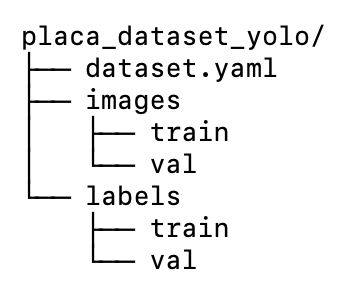
\includegraphics[width=0.20\textwidth]{figs/estructura_dataset.png}
    \caption{Estructura de directorios del dataset generado. Se organiza en carpetas de entrenamiento y validación, junto a sus respectivas anotaciones en formato YOLO.}
    \label{fig:dataset_structure}
\end{figure}

La estructura generada se muestra en la Figura~\ref{fig:dataset_structure}, donde se aprecia la separación entre datos de entrenamiento y validación, junto a sus anotaciones correspondientes.

\section{Entrenamiento de los Modelos}

Para validar la viabilidad del enfoque propuesto, se llevaron a cabo dos etapas de entrenamiento utilizando modelos basados en YOLOv7. La primera etapa consistió en entrenar un modelo segmentador de vehículos, y la segunda en entrenar un modelo segmentador de placas utilizando los datos generados automáticamente mediante el método descrito anteriormente.
\subsection{Entrenamiento del modelo de segmentación de vehículos}

Para la detección de vehículos en escenas urbanas, se entrenó un modelo YOLOv7~\cite{wang2022yolov7} empleando el conjunto de datos KITTI~\cite{geiger2012we}, el cual incluye anotaciones para objetos como \texttt{car}, \texttt{van} y \texttt{truck}. Estas tres clases fueron consideradas de forma independiente durante el entrenamiento, aunque en etapas posteriores del pipeline serán tratadas como una única categoría general (\texttt{vehículo}) para efectos de segmentación y recorte.

El entrenamiento se llevó a cabo durante 100 épocas utilizando la arquitectura base \texttt{yolov7.pt}, con tasa de aprendizaje definida en \texttt{hyp.scratch.p5.yaml}, y un tamaño de lote de 16. El proceso se realizó sobre GPU y fue monitoreado mediante la plataforma Weights \& Biases (W\&B), lo que permitió registrar y analizar la evolución de las principales métricas y funciones de pérdida.

Los resultados obtenidos reflejan una convergencia adecuada del modelo.

\begin{table}[h]
\centering
\caption{Métricas de desempeño del modelo YOLOv7 sobre el conjunto de validación (detección de vehículos).}
\begin{tabular}{lc}
\hline
\textbf{Métrica}         & \textbf{Valor} \\
\hline
Precisión               & 0.96 \\
Recall                  & 0.97 \\
mAP@0.5                 & 0.98 \\
mAP@0.5:0.95            & 0.84 \\
\hline
\end{tabular}
\label{tab:final_metrics}
\end{table}


\subsection{Entrenamiento del Segmentador de Placas (YOLOv7 sobre Dataset Generado)}

Para detectar placas dentro de recortes vehiculares, se entrenó un modelo YOLOv7 utilizando un dataset personalizado generado mediante una estrategia de detección de texto, segun el procedimiento descrito en la sección anterior. Este dataset incluye imágenes de placas peruanas con características particulares, como la palabra "PERÚ" y placas pintadas en los laterales de algunos vehículos.

El modelo fue entrenado durante 100 épocas utilizando la arquitectura \texttt{yolov7.pt}, imágenes de 640$\times$640 píxeles, tasa de aprendizaje basada en \texttt{hyp.scratch.p5.yaml}, batch de tamaño 16 y cacheo de imágenes activado. El entrenamiento fue monitorizado con W\&B.



\begin{table}[h]
\centering
\caption{Métricas de desempeño del modelo YOLOv7 sobre el conjunto de validación (detección de placas).}
\begin{tabular}{lc}
\hline
\textbf{Métrica}         & \textbf{Valor} \\
\hline
Precisión               & 0.980 \\
Recall                  & 0.992 \\
mAP@0.5                 & 0.988 \\
mAP@0.5:0.95            & 0.846 \\
\hline
\end{tabular}
\label{tab:final_metrics_plates}
\end{table}

Las gráficas obtenidas evidencian un comportamiento adecuado del modelo:



\begin{figure}[h]
\centering
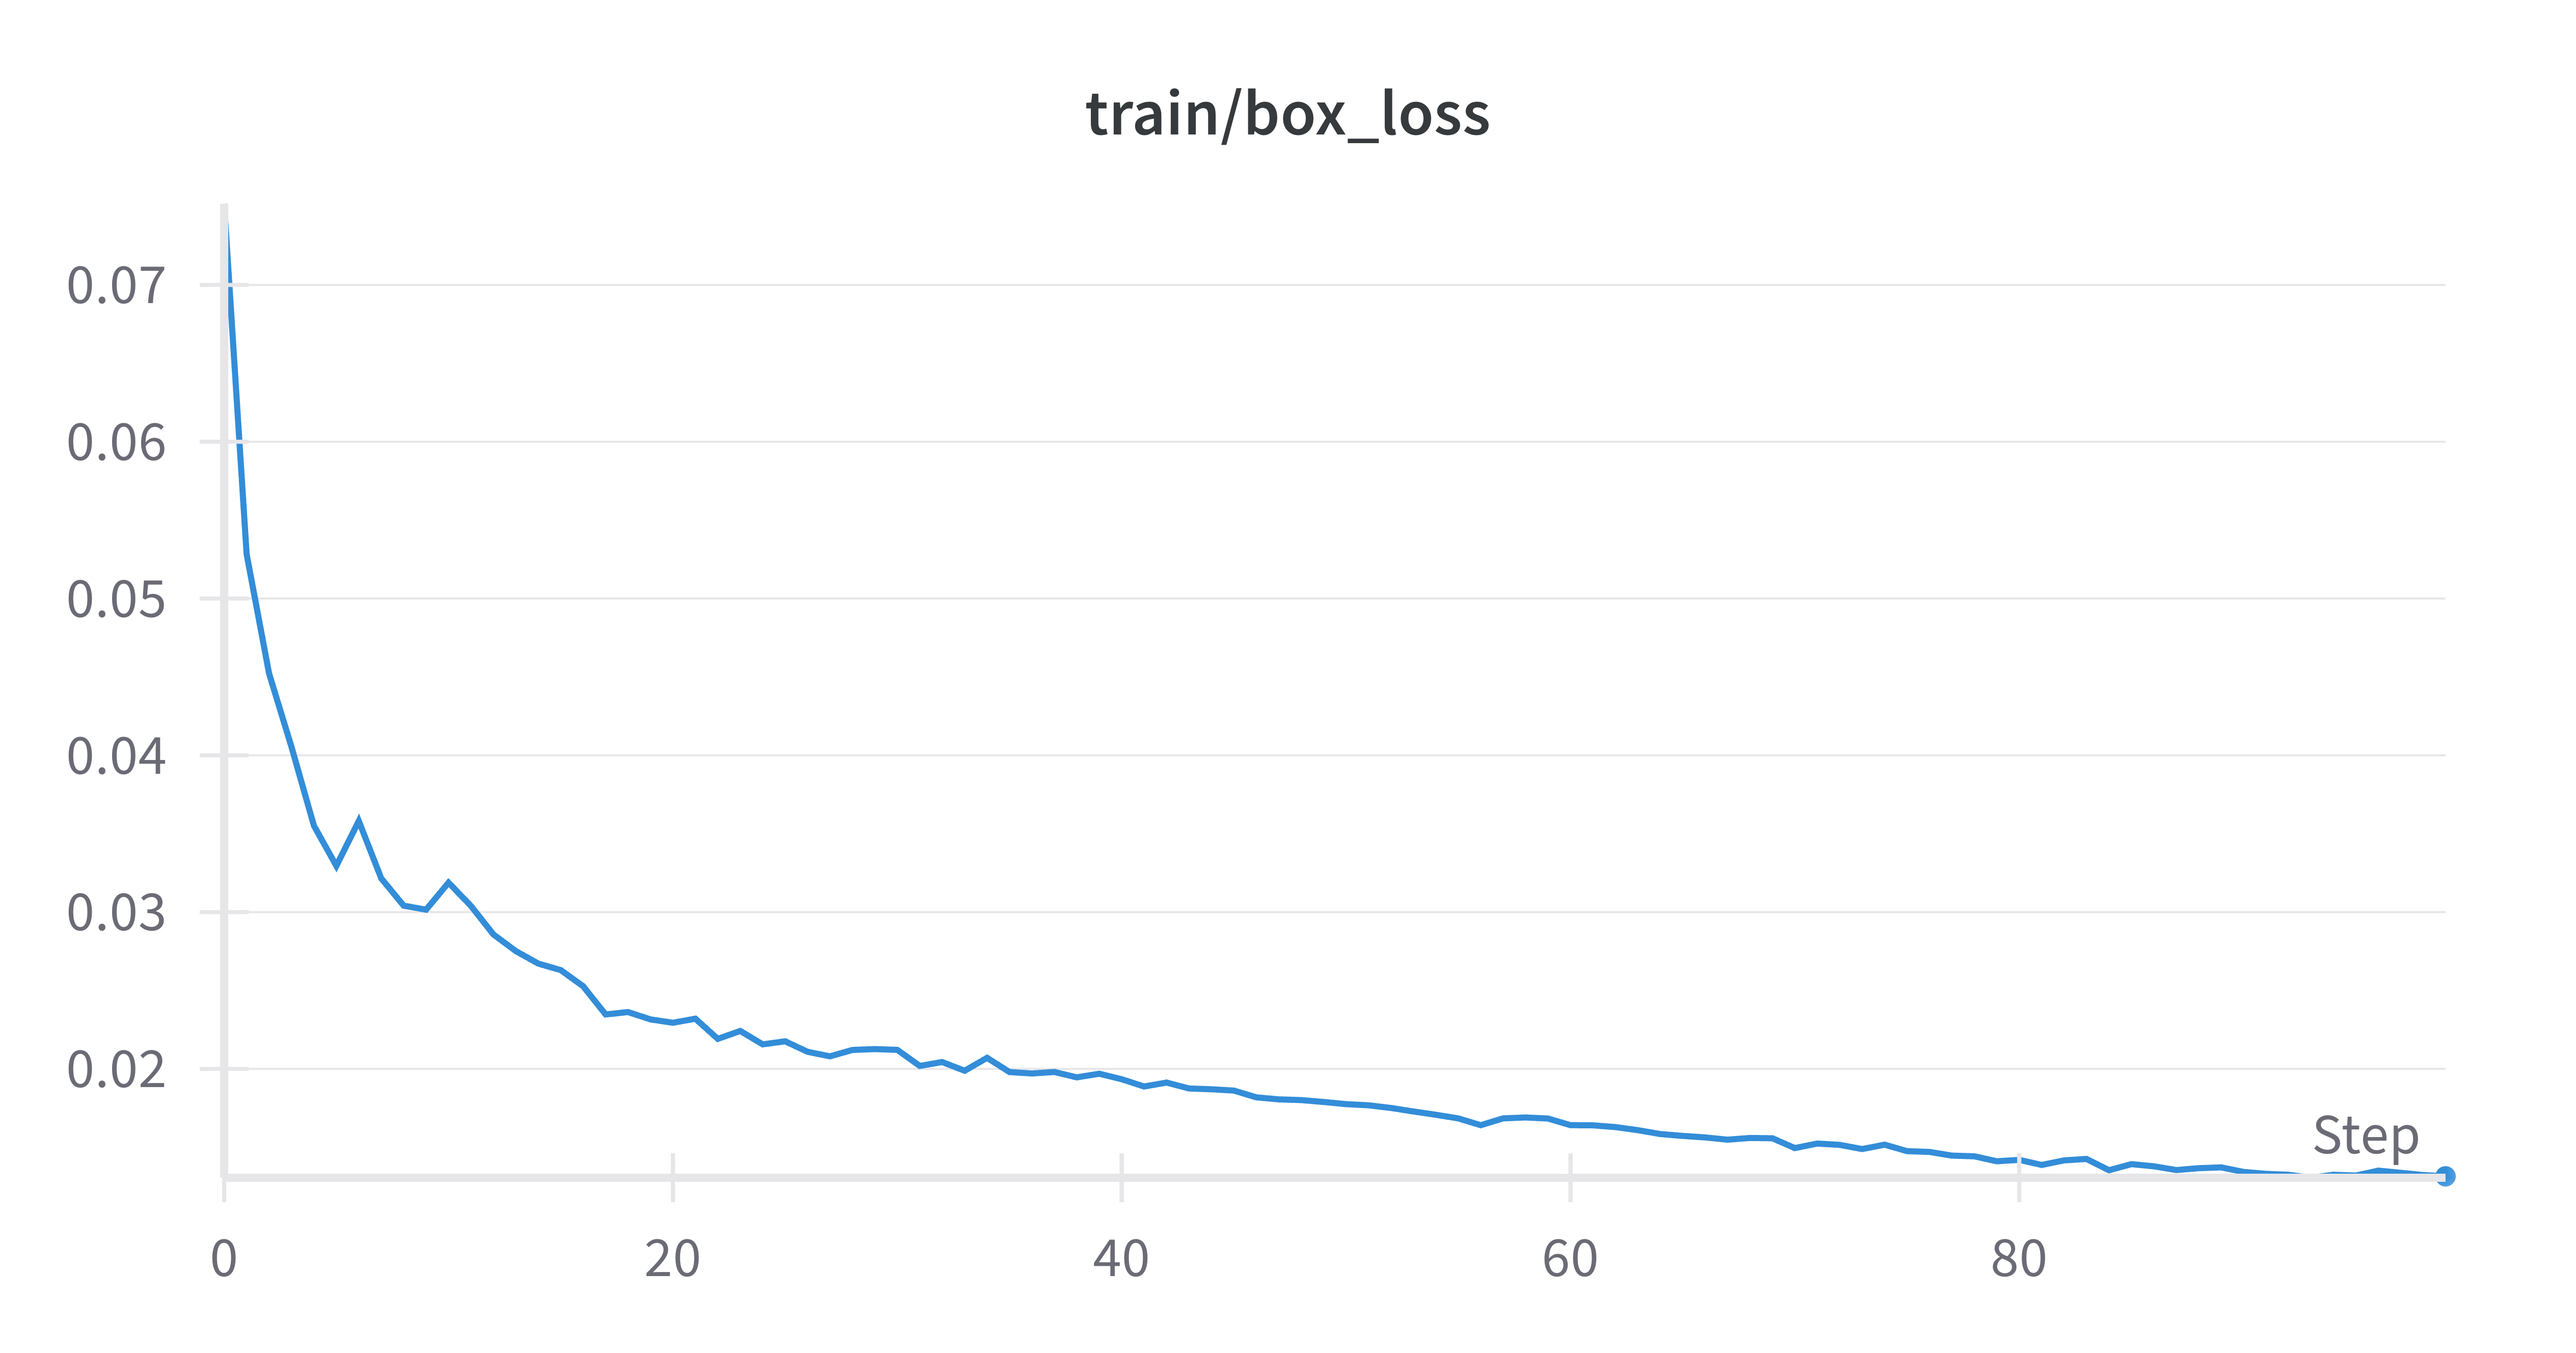
\includegraphics[width=0.45\textwidth]{figs/plate_train_box_loss.png}
\caption{Curva de pérdida de las cajas durante el entrenamiento (\texttt{train/box\_loss}).}
\label{fig:plate_train_box_loss}
\end{figure}
\texttt{train/box\_loss}: muestra una disminución sostenida, lo que indica un aprendizaje efectivo en la regresión de \textit{bounding boxes} (ver Figura~\ref{fig:plate_train_box_loss}).


\begin{figure}[h]
\centering
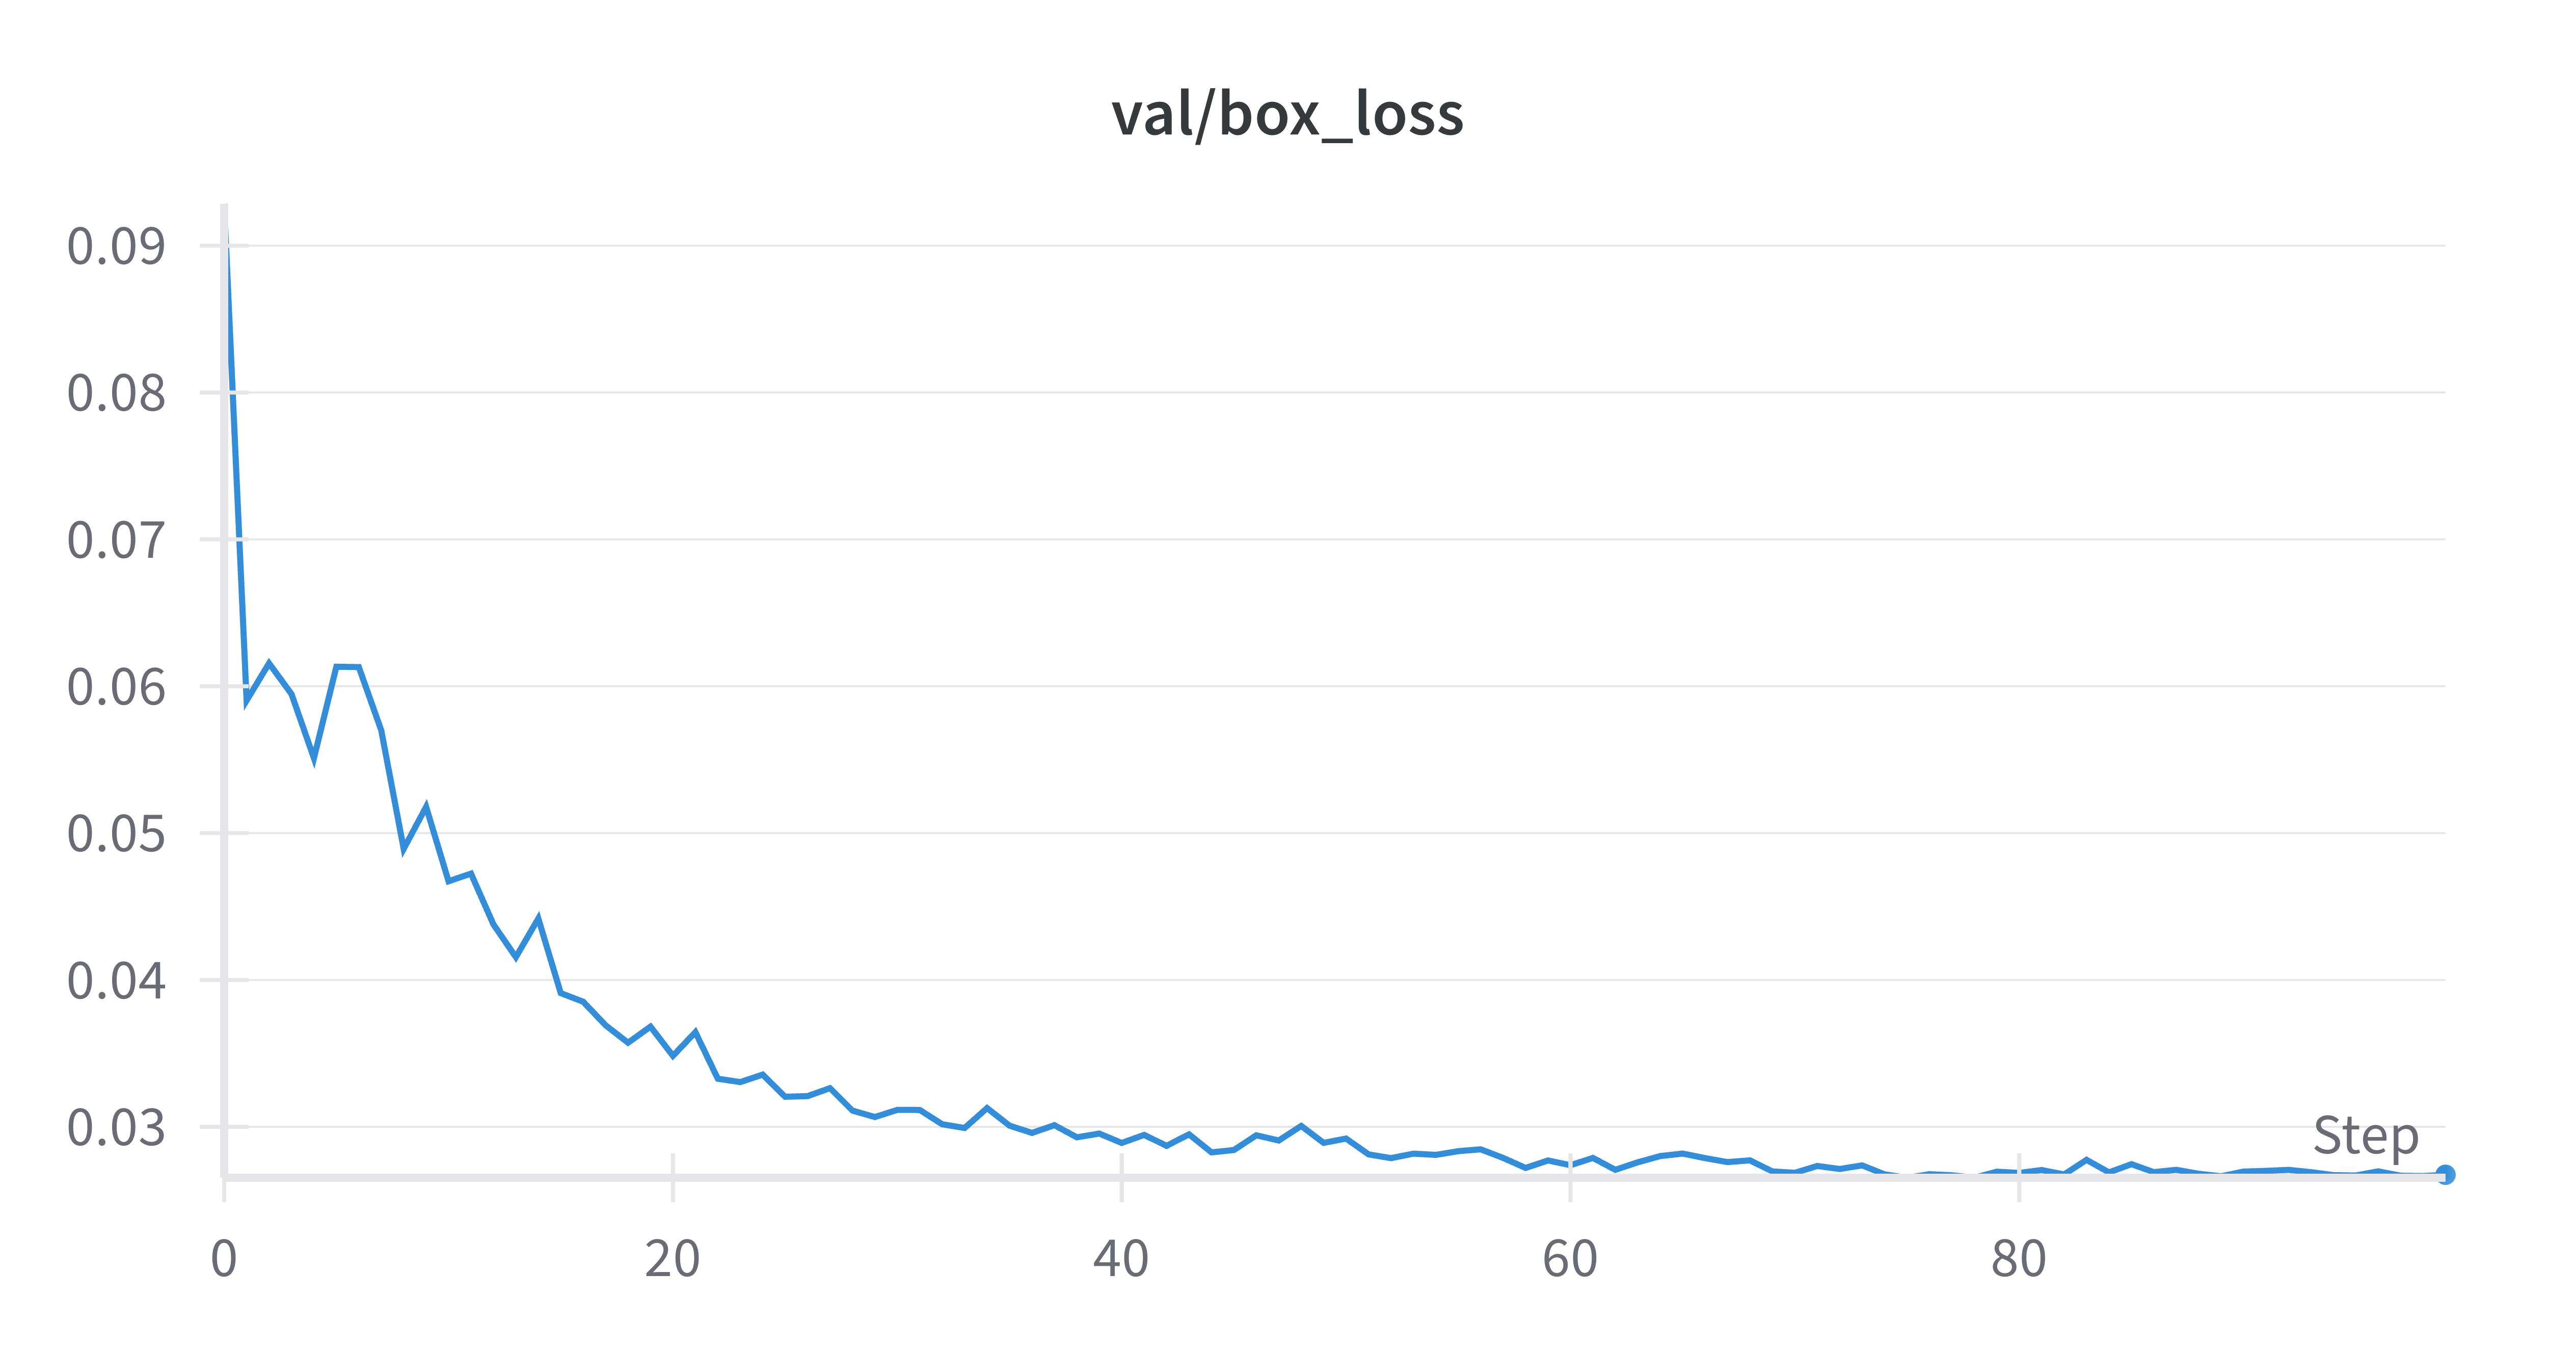
\includegraphics[width=0.45\textwidth]{figs/plate_val_box_loss.png}
\caption{Curva de pérdida de las cajas en validación (\texttt{val/box\_loss}).}
\label{fig:plate_val_box_loss}
\end{figure}
\texttt{val/box\_loss}: desciende progresivamente, lo que sugiere una correcta generalización en el conjunto de validación (ver Figura~\ref{fig:plate_val_box_loss}).



\begin{figure}[h]
\centering
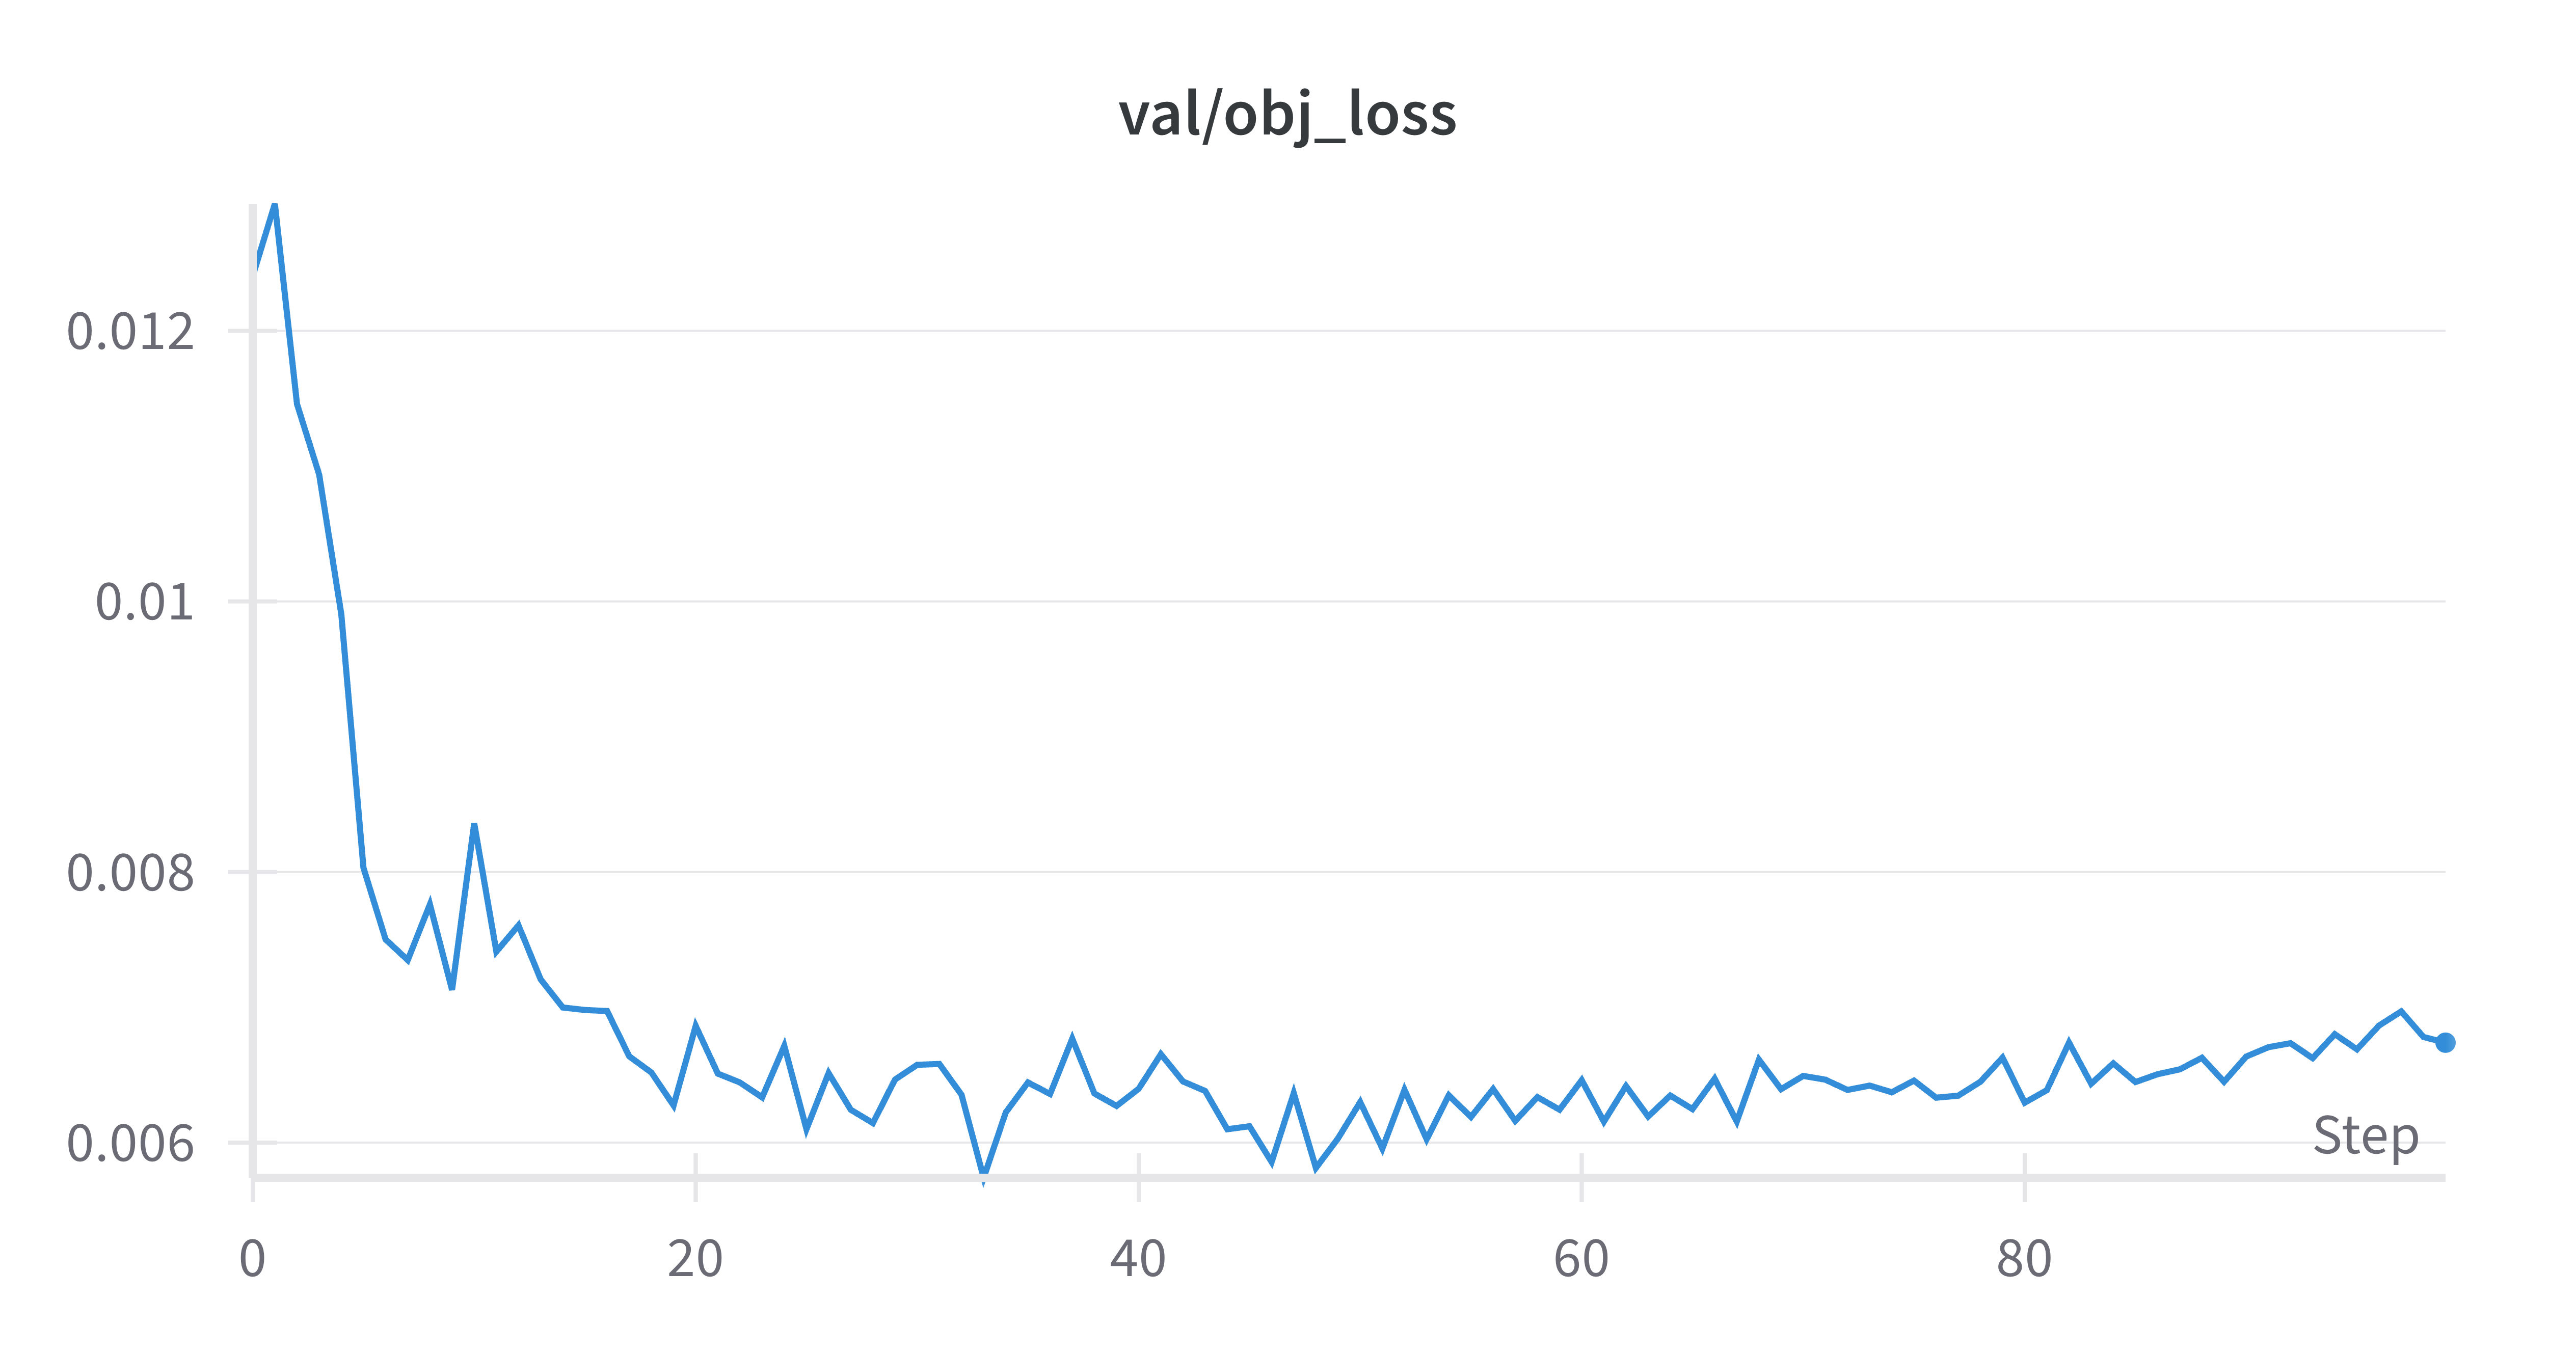
\includegraphics[width=0.45\textwidth]{figs/plate_val_obj_loss.png}
\caption{Curva de pérdida del objeto en validación (\texttt{val/obj\_loss}).}
\label{fig:plate_val_obj_loss}
\end{figure}

\texttt{val/obj\_loss}: decrece con ciertas oscilaciones y se estabiliza, lo que puede reflejar la variabilidad en las posiciones y tamaños de las placas (ver Figura~\ref{fig:plate_val_obj_loss}).

La Figura~\ref{fig:plate_val_grid} presenta una muestra de las detecciones generadas automáticamente por la plataforma W\&B al finalizar el entrenamiento. Esta visualización corresponde a una inferencia masiva del modelo segmentador sobre imágenes del conjunto de validación, permitiendo verificar de forma rápida y estructurada el rendimiento cualitativo del detector.

\begin{figure}[ht]
\centering
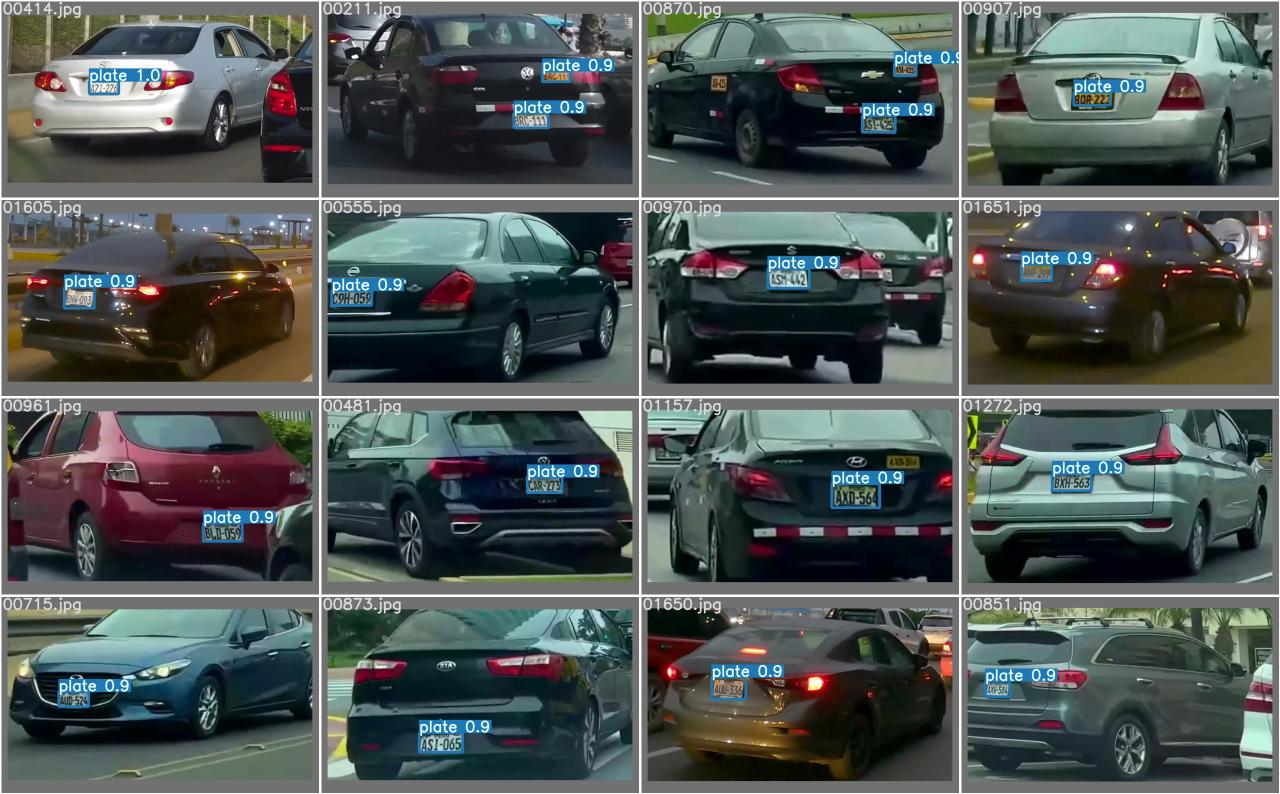
\includegraphics[width=0.45\textwidth]{figs/validation_matrix.jpg}
\caption{Grid automático de validación generado por W\&B tras la última época de entrenamiento. Se muestran predicciones sobre el conjunto de validación con sus respectivas confianzas.}
\label{fig:plate_val_grid}
\end{figure}


\section{Resultados cualitativos}

Además de las métricas cuantitativas, se presentan a continuación varios casos que ilustran el comportamiento del sistema propuesto ante situaciones reales representativas del contexto vial peruano. Estos ejemplos fueron seleccionados por su relevancia práctica y por evidenciar escenarios en los que los enfoques tradicionales suelen fallar, como la presencia de múltiples placas en un solo vehículo, placas pintadas en lugar de metálicas, o ubicaciones no convencionales.

A través de estas muestras, se busca evidenciar no solo la capacidad del modelo para detectar correctamente las placas en condiciones visuales variadas, sino también su robustez semántica al evitar falsos positivos en textos adyacentes, y su capacidad para resolver ambigüedades utilizando información redundante disponible en los vehículos (como placas duplicadas o versiones pintadas de la misma).

\begin{figure}[ht]
\centering
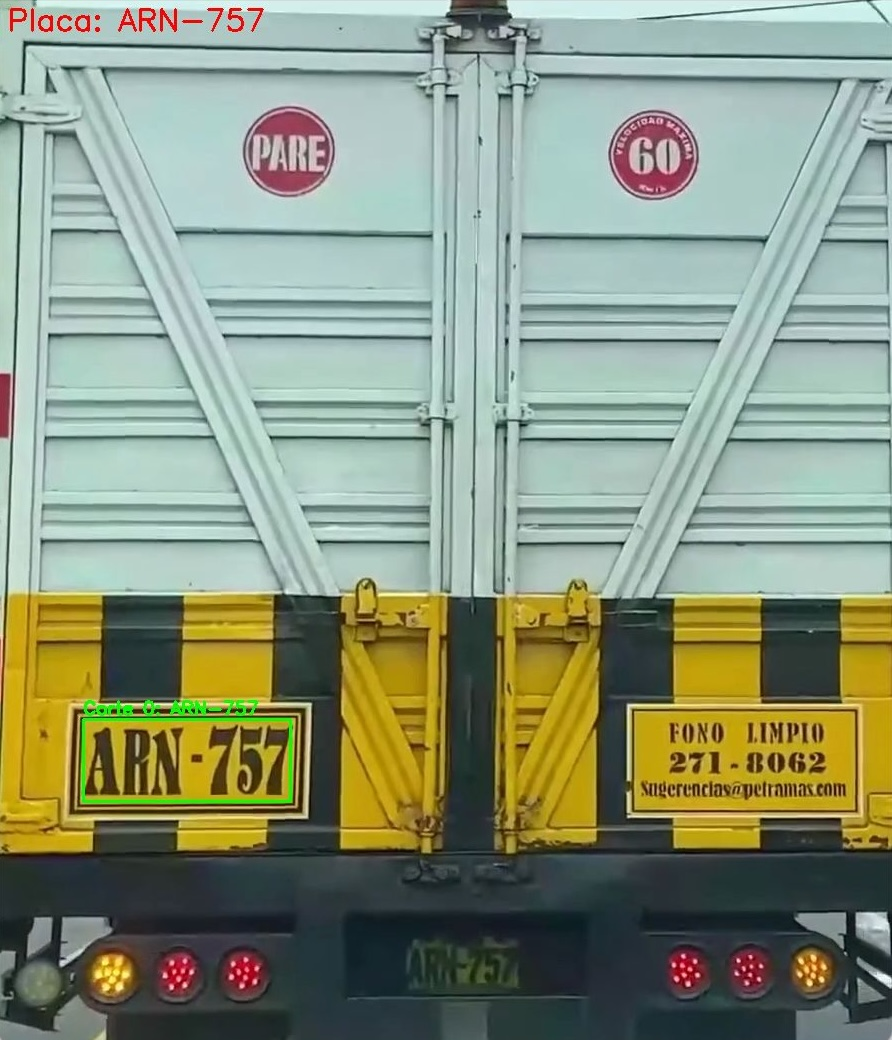
\includegraphics[width=0.35\textwidth]{figs/painted_plate_camion.jpeg}
\caption{Placa pintada detectada en un camión de carga. Aunque la placa metálica inferior es ilegible, el sistema logra identificar correctamente la versión pintada en la parte superior.}
\label{fig:painted_plate_camion}
\end{figure}

La Figura~\ref{fig:painted_plate_camion} muestra un caso frecuente en vehículos pesados del contexto peruano: la presencia de una placa pintada legible y otra metálica oscurecida o deteriorada. El enfoque propuesto permite segmentar ambas regiones, y la validación OCR prioriza la que presenta mayor confianza, contribuyendo a la robustez del sistema, es importante destacar que se discrimina la region derecha de la imagen, que corresponde a un texto no relacionado con una placa vehicular a pesar de que el estilo sea similar.

\begin{figure}[ht]
\centering
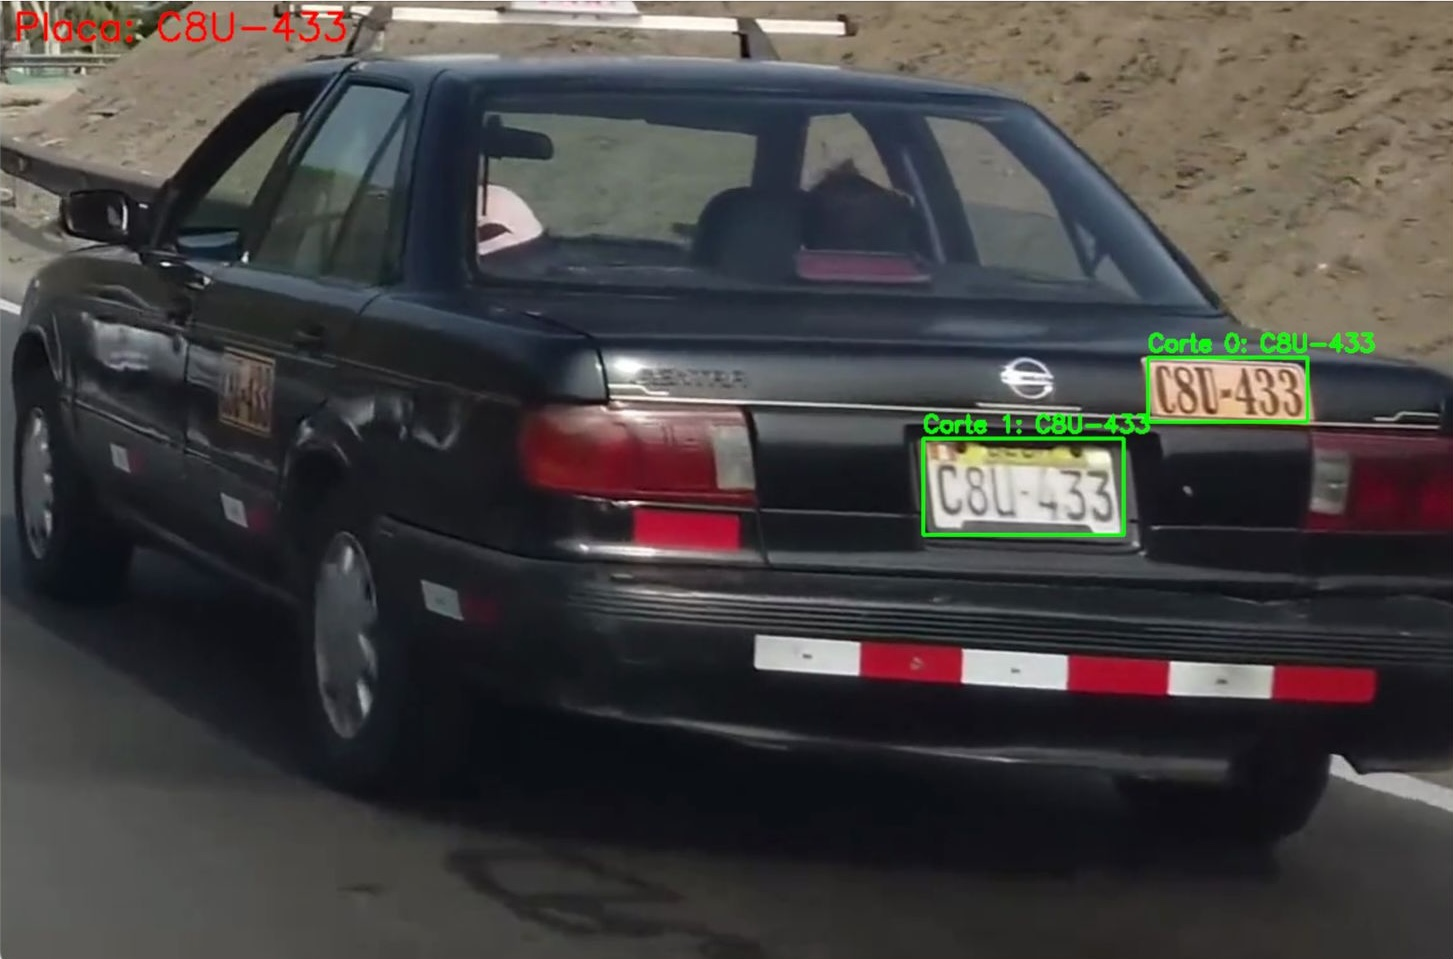
\includegraphics[width=0.35\textwidth]{figs/double_plate_taxi.jpeg}
\caption{Vehículo con doble placa (metálica y pintada). El sistema detecta ambas instancias y verifica que contienen el mismo texto, validando así la consistencia de los resultados.}
\label{fig:double_plate_taxi}
\end{figure}

La Figura~\ref{fig:double_plate_taxi} evidencia un caso donde un vehículo cuenta con dos instancias de la placa trasera, una pintada y una metálica. El modelo segmentador detecta ambas de forma independiente, y el OCR confirma su correspondencia, reforzando la fiabilidad del proceso de extracción.

\begin{figure}[h]
\centering
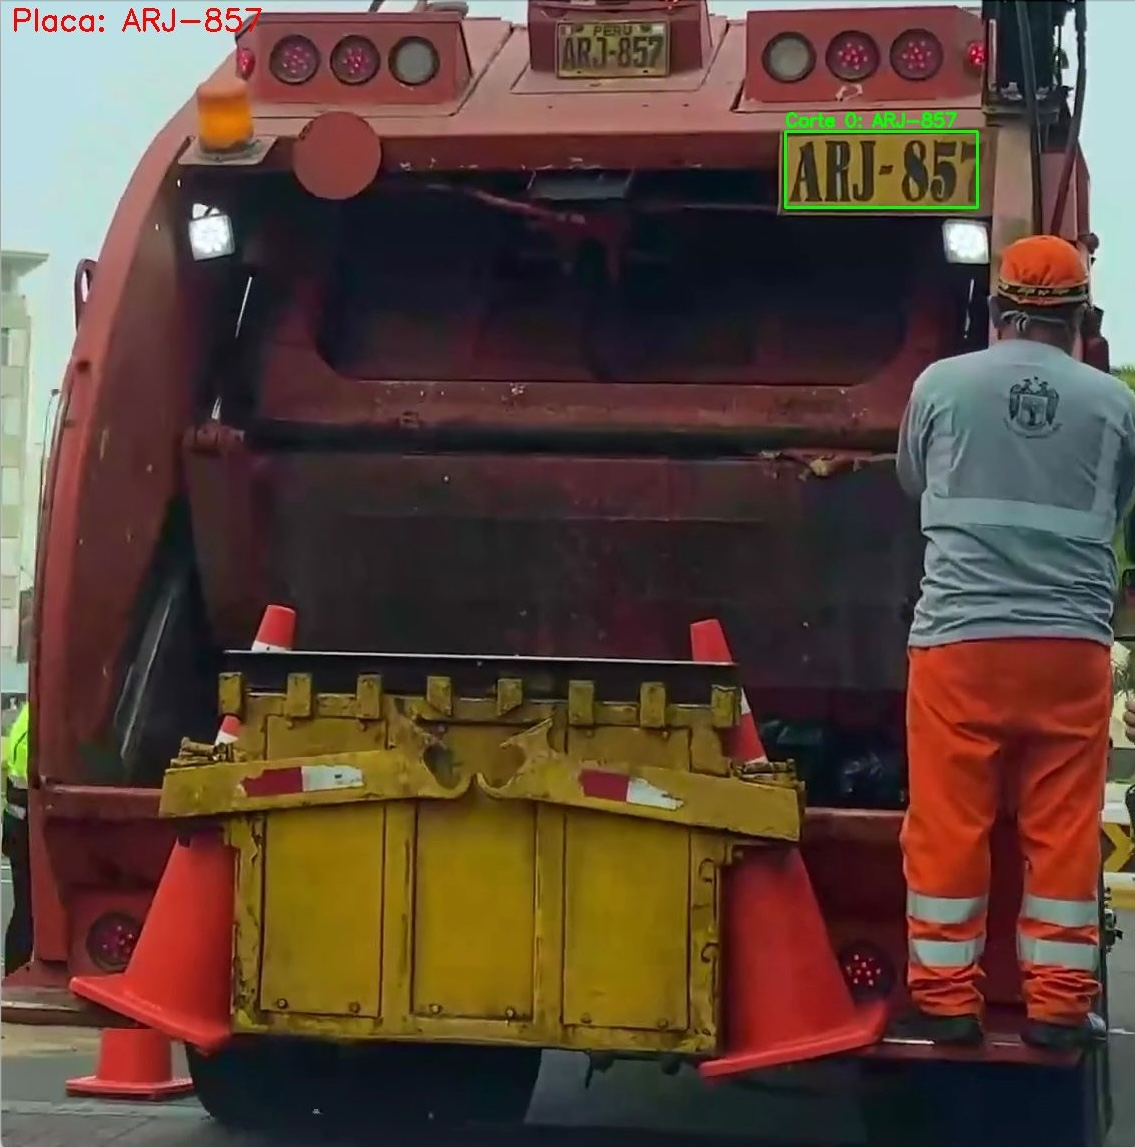
\includegraphics[width=0.35\textwidth]{figs/non_standard_plate.jpeg}
\caption{Camión recolector de residuos con placa en una ubicación no convencional.}
\label{fig:non_standard_plate}
\end{figure}

Por último, la Figura~\ref{fig:non_standard_plate} ilustra un caso poco convencional: un camión recolector de residuos cuya placa se encuentra colocada en una posición no estándar, alejada del centro inferior visual típico. A pesar del emplazamiento atípico se observa que el modelo logra detectar la placa correctamente.

\begin{figure}[ht]
\centering
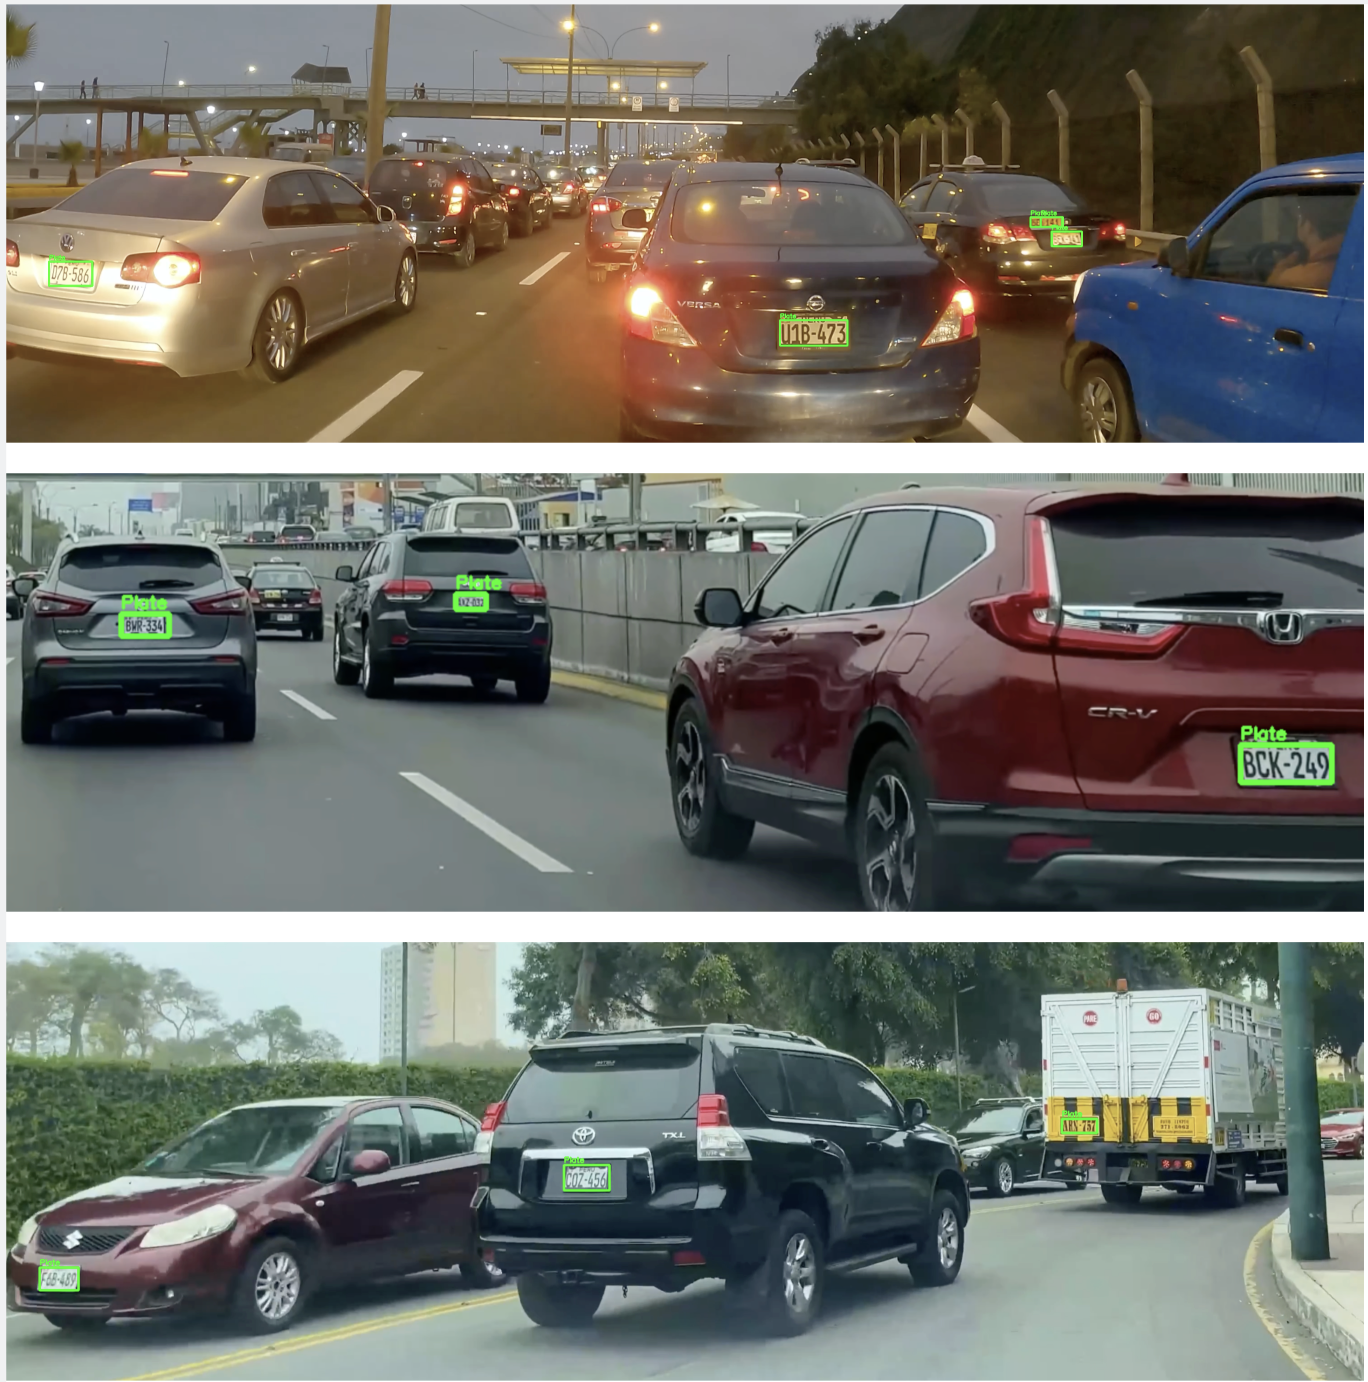
\includegraphics[width=0.48\textwidth]{figs/multi_vehicle_collage.png}
\caption{Robustez del sistema ante múltiples condiciones urbanas. Se detectan correctamente varias placas en distintos planos, horarios y tipos de vehículos, incluyendo tráfico nocturno y vehículos con placas pintadas.}
\label{fig:multi_vehicle_collage}
\end{figure}

La Figura~\ref{fig:multi_vehicle_collage} ilustra la capacidad del sistema propuesto para operar en entornos urbanos reales bajo diferentes condiciones. Se presentan escenas diurnas y nocturnas, con tráfico denso, oclusiones parciales y variedad de vehículos, incluyendo SUV, sedanes y camiones.

\section{Conclusiones}

Este trabajo presentó un enfoque robusto para el reconocimiento de placas vehiculares peruanas capturadas en condiciones reales de tránsito desde una perspectiva móvil. A diferencia de muchos modelos entrenados sobre datasets idealizados, nuestro sistema demuestra una alta capacidad de generalización ante escenas con múltiples vehículos, variabilidad en iluminación, ángulos no convencionales, y presencia de placas pintadas.

La estrategia basada en dos etapas —detección de vehículos seguida de segmentación de placas— permitió reducir significativamente los falsos positivos asociados a textos no vehiculares. La generación automatizada del dataset a partir de detección OCR validada sintácticamente, complementada con curaduría manual, garantizó la calidad del entrenamiento sin requerir costosas anotaciones desde cero.

Los resultados alcanzados por el modelo segmentador de placas, con una precisión superior al 97% y un \textit{mAP@0.5} de 0.988, respaldan la viabilidad de la propuesta para su aplicación en contextos reales, como patrullaje urbano o monitoreo embarcado.

Este trabajo podria sentar bases para futuras líneas de desarrollo que incluyan la incorporación de reconocimiento OCR end-to-end en tiempo real y la expansión del dataset con imágenes de otras regiones del país que presenten particularidades locales usando la misma tecnica de recolección y curaduría. 

\begin{thebibliography}{99}

\bibitem{xu2018towards}
Z. Xu, B. Yang, G. Zhou, X. Wang, and Y. Wu,  
“Towards end-to-end license plate detection and recognition: A large dataset and baseline,”  
\textit{arXiv preprint arXiv:1802.10130}, 2018.

\bibitem{goncalves2020ufpr}
G. P. Gonçalves, S. M. Silva, R. Laroca, E. Severo, and D. Menotti,  
“UFPR-ALPR dataset: A new dataset for Brazilian license plate recognition,”  
\textit{Iberoamerican Conference on Pattern Recognition (CIARP)}, Springer, 2020, pp. 400--408.

\bibitem{liu2024patrolvision}
W. Liu, H. Zhang, K. Tan, and C. S. Foo,  
“PatrolVision: Real-Time Vehicle License Plate Recognition System for Urban Traffic Management,”  
\textit{arXiv preprint arXiv:2504.10810}, 2024.

\bibitem{wang2022yolov7}
C.-Y. Wang, A. Bochkovskiy, and H.-Y. M. Liao,  
“YOLOv7: Trainable bag-of-freebies sets new state-of-the-art for real-time object detectors,”  
\textit{arXiv preprint arXiv:2207.02696}, 2022.

\bibitem{geiger2012kitti}
A. Geiger, P. Lenz, and R. Urtasun,  
“Are we ready for Autonomous Driving? The KITTI Vision Benchmark Suite,”  
\textit{IEEE Conference on Computer Vision and Pattern Recognition (CVPR)}, 2012, pp. 3354--3361.

\bibitem{paddleocr2020}
PaddlePaddle Team,  
“PaddleOCR: An ultra lightweight OCR system, developed by PaddlePaddle,”  
\textit{GitHub Repository}, 2020. [Online]. Available: \url{https://github.com/PaddlePaddle/PaddleOCR}. [Accessed: 05-Jun-2025].

\end{thebibliography}

\end{document}

